%%%%%%%%%%%%%%%%%%%%%%%%%%%%%%%%%%%%%%%%%
% Programming/Coding Assignment
% LaTeX Template
%
% This template has been downloaded from:
% http://www.latextemplates.com
%
% Original author:
% Ted Pavlic (http://www.tedpavlic.com)
%
% Note:
% The \lipsum[#] commands throughout this template generate dummy text
% to fill the template out. These commands should all be removed when 
% writing assignment content.
%
% This template uses a Perl script as an example snippet of code, most other
% languages are also usable. Configure them in the "CODE INCLUSION 
% CONFIGURATION" section.
%
%%%%%%%%%%%%%%%%%%%%%%%%%%%%%%%%%%%%%%%%%

%----------------------------------------------------------------------------------------
%	PACKAGES AND OTHER DOCUMENT CONFIGURATIONS
%----------------------------------------------------------------------------------------

\documentclass[a4paper]{article}

\usepackage{fancyhdr} % Required for custom headers
\usepackage{lastpage} % Required to determine the last page for the footer
\usepackage{extramarks} % Required for headers and footers
\usepackage[usenames,dvipsnames]{color} % Required for custom colors
\usepackage{graphicx} % Required to insert images
\usepackage{listings} % Required for insertion of code
\renewcommand*{\lstlistingname}{代码} % change "Listing <ref> to 代码 <ref>
\usepackage{courier} % Required for the courier font
\usepackage{lipsum} % Used for inserting dummy 'Lorem ipsum' text into the template

\usepackage[UTF8]{ctex} % Required for Chinese character
\usepackage{tocloft} % Required for beautiful toc
\usepackage[hidelinks]{hyperref} % Required for clickable toc
\hypersetup{
    colorlinks,
    citecolor=black,
    filecolor=black,
    linkcolor=black,
    urlcolor=black
}
\usepackage[title]{appendix} % Required for appendix
\usepackage{float}
\usepackage{amsmath} % used for \text{} in math formula


% used for beautiful table
\usepackage{booktabs} 
\usepackage[T1]{fontenc}
\usepackage{tabu}
\usepackage{longtable}
\usepackage[table]{xcolor}


% Margins
\topmargin=-0.45in
\evensidemargin=0in
\oddsidemargin=0in
\textwidth=6.5in
\textheight=9.0in
\headsep=0.25in

\linespread{1.1} % Line spacing

% Set up the header and footer
\pagestyle{fancy}
\lhead{\hmwkAuthorName} % Top left header
\chead{\hmwkClass\ (\hmwkClassInstructor\ \hmwkClassTime): \hmwkTitle} % Top center head
\rhead{\firstxmark} % Top right header
\lfoot{\lastxmark} % Bottom left footer
\cfoot{} % Bottom center footer
\rfoot{Page\ \thepage\ of\ \protect\pageref{LastPage}} % Bottom right footer
\renewcommand\headrulewidth{0.4pt} % Size of the header rule
\renewcommand\footrulewidth{0.4pt} % Size of the footer rule

\setlength\parindent{0pt} % Removes all indentation from paragraphs

%----------------------------------------------------------------------------------------
%	CODE INCLUSION CONFIGURATION
%----------------------------------------------------------------------------------------

\definecolor{MyDarkGreen}{rgb}{0.0,0.4,0.0} % This is the color used for comments
\lstloadlanguages{c} % Load Perl syntax for listings, for a list of other languages supported see: ftp://ftp.tex.ac.uk/tex-archive/macros/latex/contrib/listings/listings.pdf
\lstset{language=c, % Use Perl in this example
        frame=single, % Single frame around code
        basicstyle=\small\ttfamily, % Use small true type font
        keywordstyle=[1]\color{Blue}\bf, % Perl functions bold and blue
        keywordstyle=[2]\color{Purple}, % Perl function arguments purple
        keywordstyle=[3]\color{Blue}\underbar, % Custom functions underlined and blue
        identifierstyle=, % Nothing special about identifiers                                         
        commentstyle=\usefont{T1}{pcr}{m}{sl}\color{MyDarkGreen}\small, % Comments small dark green courier font
        stringstyle=\color{Purple}, % Strings are purple
        showstringspaces=false, % Don't put marks in string spaces
        tabsize=4, % 5 spaces per tab
        %
        % Put standard Perl functions not included in the default language here
        % morekeywords={rand},
        morekeywords = [1]{uint16_t, uint32_t, uint8_t, int16_t, int8_t, int32_t}
        %
        % Put Perl function parameters here
        morekeywords=[2]{on, off, interp, __attribute__},
        %
        % Put user defined functions here
        morekeywords=[3]{test},
       	%
        morecomment=[l][\color{Blue}]{...}, % Line continuation (...) like blue comment
        numbers=left, % Line numbers on left
        firstnumber=1, % Line numbers start with line 1
        numberstyle=\tiny\color{Blue}, % Line numbers are blue and small
        stepnumber=2, % Line numbers go in steps of 5,
        firstnumber=1
}

% define C style
\definecolor{main-color}{rgb}{0.6627, 0.7176, 0.7764}
\definecolor{back-color}{rgb}{0.1686, 0.1686, 0.1686}
\definecolor{string-color}{rgb}{0.3333, 0.5254, 0.345}
\definecolor{key-color}{rgb}{0.8, 0.47, 0.196}
\lstdefinestyle{mystyle}
{
    language = C++,
    basicstyle = {\small\ttfamily},
    stringstyle = {\color{Mahogany}},
    keywordstyle = {\color{blue}},
    keywordstyle = [2]{\color{Mahogany}},
    keywordstyle = [3]{\color{blue}},
    keywordstyle = [4]{\color{blue}},
    otherkeywords = {__attribute__,<<,>>,++},
    morekeywords = [2]{__attribute__},
    morekeywords = [3]{<<, >>},
    morekeywords = [4]{++, uint16_t, uint32_t, uint8_t, \#define},
}


% Creates a new command to include a perl script, the first parameter is the filename of the script (without .pl), the second parameter is the caption

\newcommand{\shfilescript}[3]{
\begin{itemize}
\item[]\lstinputlisting[caption=#2, label=lst:#1, language=sh]{#3}
\end{itemize}
}
\newcommand{\shscript}[3]{
\begin{itemize}
\item[]\begin{lstlisting}[label=lst:#1, caption=#2] #3 \end{lstlisting}
\end{itemize}
}

%----------------------------------------------------------------------------------------
%	DOCUMENT STRUCTURE COMMANDS
%	Skip this unless you know what you're doing
%----------------------------------------------------------------------------------------

% Header and footer for when a page split occurs within a problem environment
\newcommand{\enterProblemHeader}[1]{
\nobreak\extramarks{#1}{#1 见下页\ldots}\nobreak{} 
\nobreak\extramarks{接上页}{#1 见下页\ldots}\nobreak{}
}

% Header and footer for when a page split occurs between problem environments
\newcommand{\exitProblemHeader}[1]{
\nobreak\extramarks{接上页}{#1 见下页\ldots}\nobreak{}
\nobreak\extramarks{#1}{}\nobreak{}
}
% TODO:code here enable the number before section, but it disable the numbering of problems
%\setcounter{secnumdepth}{0} % Removes default section numbers
\newcounter{homeworkProblemCounter} % Creates a counter to keep track of the number of problems

\newcommand{\homeworkProblemName}{}

\newenvironment{homeworkProblem}[1][Problem \arabic{homeworkProblemCounter}]{ % Makes a new environment called homeworkProblem which takes 1 argument (custom name) but the default is "Problem #"
\stepcounter{homeworkProblemCounter} % Increase counter for number of problems
\renewcommand{\homeworkProblemName}{#1} % Assign \homeworkProblemName the name of the problem
\section{\homeworkProblemName} % Make a section in the document with the custom problem count
\enterProblemHeader{\homeworkProblemName} % Header and footer within the environment
}{
\exitProblemHeader{\homeworkProblemName} % Header and footer after the environment
}

\newcommand{\problemAnswer}[1]{ % Defines the problem answer command with the content as the only argument
\noindent\framebox[\columnwidth][c]{\begin{minipage}{0.98\columnwidth}#1\end{minipage}} % Makes the box around the problem answer and puts the content inside
}

\newcommand{\homeworkSectionName}{}
\newenvironment{homeworkSection}[1]{ % New environment for sections within homework problems, takes 1 argument - the name of the section
\renewcommand{\homeworkSectionName}{#1} % Assign \homeworkSectionName to the name of the section from the environment argument
\subsection{\homeworkSectionName} % Make a subsection with the custom name of the subsection
\enterProblemHeader{\homeworkProblemName\ [\homeworkSectionName]} % Header and footer within the environment
}{
\enterProblemHeader{\homeworkProblemName} % Header and footer after the environment
}


\newcommand{\codev}[1]{\textsf{#1}}
%----------------------------------------------------------------------------------------
%	NAME AND CLASS SECTION
%----------------------------------------------------------------------------------------

% table color
\definecolor{tableHeader}{RGB}{245, 245, 245}
\definecolor{tableLineOne}{RGB}{245, 245, 245}
\definecolor{tableLineTwo}{RGB}{224, 224, 224}
\newcommand{\tableHeaderStyle}{
    \rowfont{\leavevmode\color{white}\bfseries}
    \rowcolor{tableHeader}
}

%----------------------------------------------------------------------------------------

\newcommand{\hmwkTitle}{操作系统原理实验\ \#3} % Assignment title
\newcommand{\hmwkDueDate}{Monday,\ April\ 2,\ 2018} % Due date
\newcommand{\hmwkClass}{16级计科\ 7班} % Course/class
\newcommand{\hmwkClassTime}{周一9-10节} % Class/lecture time
\newcommand{\hmwkClassInstructor}{凌应标} % Teacher/lecturer
\newcommand{\hmwkAuthorName}{颜彬} % Your name
\newcommand{\hmwkAuthorId}{16337269} % Your id 

%----------------------------------------------------------------------------------------
%	TITLE PAGE
%----------------------------------------------------------------------------------------

\usepackage{titling}

\title{
\vspace{2in}
\textmd{\textbf{\hmwkClass:\ \hmwkTitle}}\\
\normalsize\vspace{0.1in}\small{Due\ on\ \hmwkDueDate}\\
\vspace{0.1in}\large{\textit{\hmwkClassInstructor\ \hmwkClassTime}}
\vspace{3in}
}

\author{\textbf{\LARGE{\hmwkAuthorName}} \\ \\ \textbf{\LARGE{\hmwkAuthorId}}}
\date{} % Insert date here if you want it to appear below your name
%----------------------------------------------------------------------------------------

\begin{document}
% \begin{titlingpage} % This is for ignore page number in first page. package titling

\maketitle

%----------------------------------------------------------------------------------------
%	TABLE OF CONTENTS
%----------------------------------------------------------------------------------------

% \setcounter{tocdepth}{2} % Uncomment this line if you don't want subsections listed in the ToC
% set depth in toc

% \renewcommand{\cftsecleader}{\cftdotfill{\cftdotsep}} % used for dots between <section> and <page>

\renewcommand{\contentsname}{Content} % force the word to be "content
\newpage
\tableofcontents
\addtocontents{toc}{~\hfill\textbf{Page}\par}
\newpage

% below are document body


% To have just one problem per page, simply put a \clearpage after each problem
\section{实验目的}
把原来在引导扇区中实现的监控程序(内核)分离乘一个独立的执行体,存放那个在其他扇区中,为``后来''扩展内核提供发展空间。\\

学习汇编与C混合编程技术,改写实验二的监控程序,拓展其命令处理能力,增加实现实验要求2中的部分或全部要求。
\section{实验要求}
在实验二的基础上进行,保留或拓展原有功能,实现部分新增功能。\\

监控程序以独立的可执行程序实现,并由引导程序加载进内存适当位置,内核获得控制权后开始显示必要的操作提示信息,实现若干命令,
方便使用者(测试者)操作。\\

制作包包含引导程序,监控程序和若干可加载并执行的用户程序组成的1.44M软盘映像。\\

\section{实验方案}
    \subsection{基础原理}
    \subsubsection{GCC与NASM的合作}\label{subsec:GccNasmHybrid}
    计算机本质上只能运行对应架构的机器码。C程序和汇编程序在运行时,都是先通过编译器将源码生成目标文件,
    再用链接器将若干个(或一个)目标文件链接成可执行文件(或纯二进制文件)。由于C语言生成的目标文件和汇编
    语言生成的目标文件本质上是一样的,这就允许我们将来自C和汇编的目标文件通过链接器连在一起,生成混编可执行文件。\\
    
    实验一、二实质上是使用32位处理器的16位模式执行16位代码。NASM产生的汇编的立即数和地址都是16位的。
    然而GCC只能产生32位的代码。如果强行将16位汇编和32位GCC汇编连接,会在运行时出现问题。32位GCC汇编的
    立即数都是32位的,处理器会读取32位立即数的低16位作为立即数,把立即数的高16位看作是``下一条指令的代码''。\\

    幸运的是,我们使用的处理器是32位的(只是模式是16位),其可以用某种方式处理32位代码:如果一个条汇编语句带有
    前缀``66'',处理器明白这条语句的立即数长度``与当前模式不一致''。由于当前模式是16位,故处理器知道这条语句的立即数
    是32位的。处理器在识别立即数时可以往后读取32个比特。类似地,前缀67表示``地址''长度与默认模式不一致。66,67前缀可以
    理解成,告诉处理器``暂时地''切换到32位模式执行当前代码。 \\

    GCC的编译选项 $-m16$ 可以自动地在所有(必要的)指令前加前缀66,67。如此处理器即可正确地处理立即数长度和
    地址长度。注意到,$-m16 $ 相当于在C代码的最开头内嵌一条汇编语句$.code16gcc$。显然采用编译指令的方式比手动
    内嵌汇编指令方便得多。\\
    
    所有的编译参数见\ref{subsec:gccCompileIns}。 \\
    
    GCC和NASM有一个很重要的技术细节,忽略将会产生严重的错误,见\ref{subsec:gccnamspitfall}节。
   
    混编时运用内嵌汇编可以简化程序代码的书写。见第\ref{subsec:inlineasm}小节。
    \subsubsection{链接器的作用}
    由于我们还无法实现解析EXE头和ELF头,所以连接器应增加$-oformat \  binary$参数,以保证最终产生不带头的二进制文件。\\
    
    在混编中,链接器代替了以前的$ORG$伪指令的作用。当然,因为链接器需要全权负责地址偏移量的计算,所以链接器不允许
    代码内出现任何的$ORG$,否则将报错。\\
    
    所有汇编程序先删除所有的$ORG$伪指令。在链接时通过$-Ttext\ <address>$的方式决定代码段的偏移量。\\
    
    链接主引导程序时,使用$-Ttext\ 0x7C00$参数。 \\

    链接操作系统引导时,使用$-Text\ 0x7E00$参数。此处假设主引导会把操作系统引导
    载入到内存0x7E00处。\\ 
    
    链接操作系统内核时,使用$-Text\ 0xA200$参数。此处假设主引导会把内核载入0xA200处。\\ 

    所有的链接参数见 \ref{subsec:LDIns}节。
    \subsubsection{FAT文件系统}\label{subsec:filesystem_intro}
    本实验还实现了简单的FAT16文件系统,提供了若干接口,并完成了列出当前目录$ls$, 运行文件$run$,以及简单的文件权限检查等操作。
    操作系统引导借助文件系统的接口,在根目录下搜索kernel.bin文件,并将其载入到内存中。\\
    
    在开机后,主引导程序首先将控制权交给操作系统引导程序。操作系统引导会从查找BPB表,找到第一个FAT表所在扇区和FAT表长度
    ,把FAT表加载入内存;还会找到数据块区中的``根目录区'',把它也载入到内存中。
    随后,操作系统引导会调用文件系统提供的接口,搜索根目录的前5个文件,查看其是否为kernel.bin。\\
    
    当操作系统引导找到根目录区中的kernel.bin项后,它会找到该项的$cluster$和$file\ size$。引导会再次读取BPB表,
    找到该$cluster$所在扇区,计算内核的扇区数,把相关扇区载入到内存中。随后,操作系统引导将控制权交给内核。\\
    
    至此,所有引导工作全部完成。内核接管所有的控制权。文件系统的布局图见\ref{fig:FAT16layout}.
    \subsubsection{混编的坑点}\label{subsec:gccnamspitfall}
    第\ref{subsec:GccNasmHybrid}节讨论了GCC和NASM混编的可行之处。但在细节上,它们的混编还有一个不易被留意的坑点。
    不注意的话,会导致程序完全错误。\\
    
    GCC产生的汇编本质是32位的,GCC编译出的函数在call时,会向栈中压入32位地址。若C函数调用(16位)汇编,汇编的ret指令
    只会出栈16位地址。在大部分情况下,这个错误不会被发现:因为32位的地址的高16位一般是0,只依靠低16位就可以正确跳转。但
    这个错误会带来极其严重的后果。栈指针在调用函数后没有返回到正确的值中。栈中被压入了多余的16个0.随后的所有访问栈操作都会
    发生错误。\\
    
    解决这个问题的方法很简单。如代码\ref{lst:workaround}所示。用pop ecx; ret cx的方式,手动出栈32个字节,并跳转ecx
    的低16个字即可。为了便于以后的代码书写,代码\ref{lst:workaround}把这几行代码定义成了宏。例如pushl和calll将执行
    32位的入栈和函数调用操作。retl将执行32位的函数返回操作。
    \subsubsection{内嵌汇编的书写}\label{subsec:inlineasm}
    GCC支持C程序中内嵌汇编。这给编程带来了很大的帮助。例如操作系统内核kernel.c在开头内嵌了代码\ref{lst:asminclude}所示的汇编。\\
    
    开头的.globl \_start和\_start:的作用是告知链接器程序的入口地址。第3-5行代码把ds和es设置为0,做了一些简单的初始化工作。
    最后一行的jmpl \$0, \$main 直接跳转到main函数。这样,无论kernel.c在main函数前定义了多少数据、函数,都可以保证程序在执行时
    能第一时间跳转到main函数,避免执行错误的代码和数据。\\
    
    \_\_asm\_\_语法也支持采用intel汇编来书写。方法是,采用\_\_asm\_\_(".intel\_syntax noprefix\\n");。需要注意的是,
    在内嵌汇编执行完后,要手动把语法再改成at\&t语法,否则其后的所有(GCC生成的)汇编无法正确工作。方法是,\_\_asm(".att\_syntax\\n")\_\_;

    \begin{figure}[!hbt]
    \begin{itemize}
    \item[] \begin{lstlisting}[language={[x86masm]Assembler}, label=lst:asminclude, caption=kernel.c文件头包含的内嵌汇编]
__asm__(".globl _start\n");
__asm__("_start:\n");
__asm__("mov $0, %eax\n");
__asm__("mov %ax, %ds\n");
__asm__("mov %ax, %es\n");
__asm__("jmpl $0, $main\n");
    \end{lstlisting}
    \end{itemize}
    \end{figure}

    \begin{figure}[!hbt]
    \begin{itemize}
    \item[] \begin{lstlisting}[language={[x86masm]Assembler}, label=lst:workaround, caption=解决函数调用时地址长度不一致的问题]
; in file /include/bridge.inc
%macro pushl 1
    push word 0
    push word %1
%endmacro

%macro calll 1
    push word 0
    call %1
%endmacro

%macro retl 0
    pop ecx
    jmp cx

%endmacro
    \end{lstlisting}
    \end{itemize}
    \end{figure}
    \subsection{实验环境}
    \subsubsection{系统与虚拟机}
    \begin{itemize} \item 操作系统 \\ 
        本实验在Linux下完成。采用Ubuntu 16.04
        \item 虚拟机\\
        bochs.它是一款开源且跨平台的 IA-32 模拟器。
    \end{itemize}
    \subsubsection{相关工具、指令}
        \begin{itemize}
            \item 汇编器\\ 
            NASM. NASM是一个轻量级的、模块化的 80x86 和 x86-64 汇编器。它的语法与
            Intel 原语法十分相似,但更加简洁和易读。它对宏有十分强大的支持。
            \item 编译器\\
            GCC. GNU/GCC 是开源的C语言编译器。其产生的伪16位代码可以与NASM结合,混编生成伪16位程序。
            \item 镜像文件产生工具\\ 
            bximage. 该命令允许生成指定大小的软件镜像。
            \item 二进制写入命令\\ 
            dd. dd 允许指定源文件和目标文件,将源文件的二进制比特写入目标文件中的指定位置。
            \item 二进制文件查看命令\\ 
            xxd. xxd 允许将二进制文件中的内容按地址顺序依次输出,可读性强
            \item 反汇编器\\
            objdump. objump可以查看目标文件和二进制文件的反汇编代码,还能指令intel或at\&t格式显示。
            \item 代码生成脚本\\
            makefile. makefile脚本具有强大的功能,其可以识别文件依赖关系,自动构筑文件,自动执行shell脚本等。
        \end{itemize}
    \subsection{程序流程}\label{subsec:programProcedure}
    文件系统在虚拟软盘中的镜像如图\ref{fig:FAT16layout}。全部引导的简要过程见图\ref{fig:loading}。
    
    \begin{figure}
        \begin{center}
        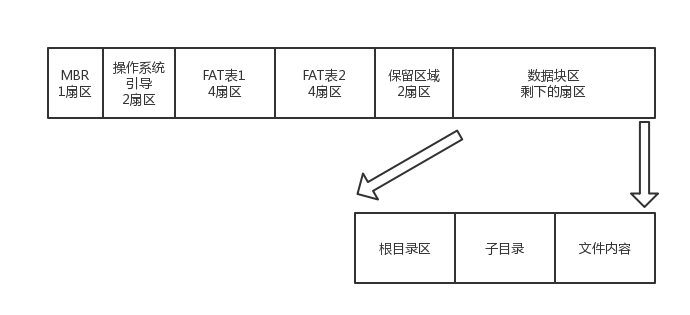
\includegraphics[scale=0.5]{asset/softImage.png}
        \caption{FAT16文件系统布局\label{fig:FAT16layout}} 
        \end{center} 
    \end{figure} 
    
    
    \begin{figure}
        \begin{center}
        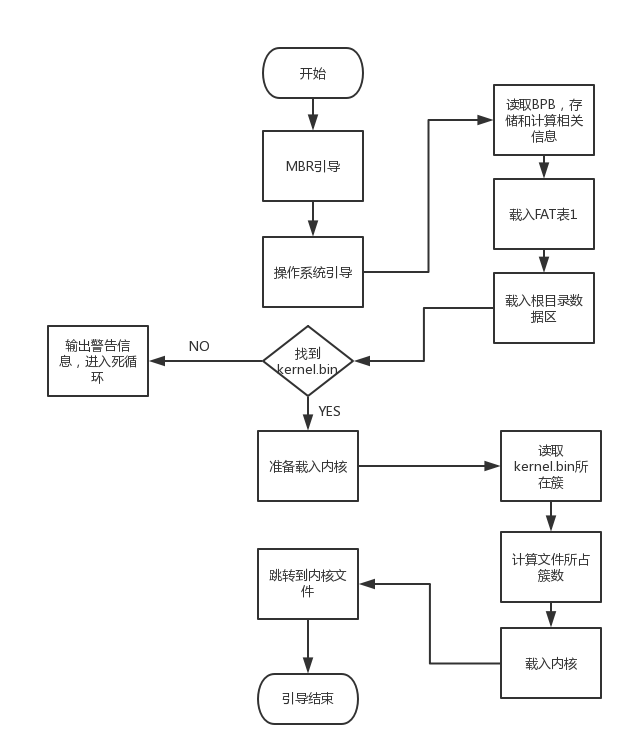
\includegraphics[scale=0.6]{asset/loading.png}
        \caption{引导内核的全过程\label{fig:loading}} 
        \end{center} 
    \end{figure} 
    
\section{实验过程}
    \subsection{项目目录树介绍}\label{sec:pjtree}
    项目的目录树见代码\ref{lst:pjtree}。\\
    
    filesystem/\\
    存放的Models是与文件系统实现相关的文件。其中操作系统引导程序也放在这个目录下。
    这是由于操作系统引导与文件系统密切相关。/filesystem/API/存放的是文件系统接口。
    用户程序只需include接口即可使用文件系统的相关功能。\\
    
    include/\\
    存放的是内核、用户程序都可能需要的代码。其中包括打印函数、清屏函数、字符串处理函数等。\\
    
    kernel/\\
    存放的是内核程序。\\
    
    loader/\\
    存放的是主引导程序。\\
    
    user/\\
    存放的是用户程序。其中本项目还实现了简单的终端。终端程序也作为用户程序放在此处。user/stone/存放
    的是项目一、二的stone程序。\\
    
    详细的整个目录树见附录\ref{sec:otherCode}代码\ref{lst:wholepjtree}。
    \begin{figure}[!hbt]
    \begin{itemize}
    \item[] \begin{lstlisting}[label=lst:pjtree, caption=项目目录树介绍(仅文件夹)]
.
|-- filesystem/
|   |-- API/
|-- include/
|-- kernel/
|-- loader/
|-- user/
    |-- stone/

7 directories
    \end{lstlisting}
    \end{itemize}
    \end{figure}
    \subsection{构建GCC+NASM混编的全部指令}
    本项目采用$makefile$构筑。本项目按照\ref{sec:pjtree}节讲述的方式分成若干子文件夹。每个子
    文件夹中都有各自的$Makefile$文件。整体的$Makefile$会分别调用各个子文件夹中的$Makefile$,最终
    构建出整个项目。
    \subsubsection{GCC编译指令} \label{subsec:gccCompileIns}
    所有的C程序都采用了表\ref{tab:gcc}所示的编译指令。

    \begin{table}[!htb]
        \caption{GCC编译指令}\label{tab:gcc}
    \begin{tabular}{@{} *5l @{}} 
        \toprule
    \emph{编译选项} & \emph{作用} &&&  \\
        \midrule
        -o    & D  \\ 
        \\ 
        -march=i386  & X产生原始Itel i376 CPU架构的代码\\ 
        \\
        -m16& 等价于汇编伪指令.code16gcc。
            \\& 在所有必要的指令前加,前缀66, 67,
            \\& 使得处理器能以32位的方式读取GCC产生的代码\\
        \\
        -mpreferred-stack-boundary=2 & 以$2^i$bytes作为对齐量,对齐栈的界限。
            \\& 该选项默认为4(即默认$2^4$字节对齐栈界限).
            \\& 为了节省空间,这里设置成2 \\
        \\
        -ffreestanding &  产生``自立''的程序文件.
            \\& 即告知GCC不使用(几乎)所有的库头文件。
            \\& 保证产生的代码不依赖于GCC的自带库 \\
        \\
        -c & 不产生可执行文件,只执行``编译''操作产生目标文件 \\ 
        \\
        -Og & 产生最小限度的优化.
            \\& 即这个优化能化简汇编代码,但又
            不影响汇编程序的可读性。\\
        \\
        -O0 & 不产生任何优化。
            \\& 本项目文件系统FAT表的构建使用C语言的struct
            完成。
            \\& 为了保证产生的二进制表项和C代码中的struct严格一致
            \\& 必须
            采用本优化等级。\\

        \bottomrule
    \hline
    \end{tabular}
    \end{table}
    \subsubsection{LD链接指令}\label{subsec:LDIns}
    目标文件在链接时采用表\ref{tab:ld}所示的指令。
    \begin{table}[!hbt]
        \caption{LD链接指令}\label{tab:ld}
    \begin{tabular}{@{} *5l @{}}    
        \toprule
    \emph{LD链接器选项} & \emph{解释} &&&  \\
        \midrule
        -melf\_i386    & 链接成intel 386架构的代码 \\ 
        \\ 
        -N & 关闭页对齐。禁止链接动态库。\\
        \\
        -oformat binary & 产生纯二进制文件,即不带文件头 \\
        \\
        -Ttext 0xA200 & 设text段(代码段)的偏移量为0xA200。
            \\& 同理还有Tbss, Tdata等。 \\
        \bottomrule
    \hline
    \end{tabular}
    \end{table}

    \subsection{文件系统} \label{sec:fsapi}
    \subsubsection{文件系统API}
    文件系统提供了以下的API供内核和用户程序调用。操作系统主引导在
    载入内核时需要搜索$kernel.bin$,也是采用这套接口完成搜索。\\

    文件系统实现了最基本的功能,例如搜索文件,进入文件夹,将文件从
    软盘载入内存中,执行文件等。但修改操作还未实现。所以不支持写文件
    和删除文件.\\ 

    由于考虑到进程控制块还未实现,系统的其他部分也都很简陋,故没有实现``文件描述符''
    层次的API接口。只实现了很底层的接口,供内核暂时调用。\\
    
    函数开头都带有双下划线,暗示这是系统的底层接口。以后实现的高层接口不会带有双下划线。
    \begin{table}[!htb]
    \caption{FAT16文件系统接口 }\label{tab:fatAPI}
    \begin{tabular}{@{} *5l @{}}
        \toprule
    \emph{函数声明} & \emph{功能} &&& \\
        \midrule
        FAT\_ITEM & FAT\_ITEM是一个类型
            \\& 位于datablock中的长32字节的结构(表项)\\
        \\
        FAT\_ITEM* \_\_get\_root\_dir() & 返回根目录表项 \\
        \\
        int16\_t \_\_next\_item(const FAT\_ITEM* p) 
            & 返回当前指针指向的下一个表项
            \\& 该函数能自动跳过被删除的表项 \\
        \\
        int16\_t \_\_has\_next\_item(const FAT\_ITEM* p)
            & 判断当前指针是否还有下一表项
            \\& 返回0和1分别代表false和true
            \\& 自动跳过被删除的表项 \\
        \\
        int16\_t \_\_FAT\_item\_type(const FAT\_ITEM* p)
            & 返回指针指向表项的类型
            \\& 例如文件、文件夹、系统文件等
            \\& 文件类型有一套宏定义,增加可读性 \\
        \\
        FAT\_ITEM* \_\_jump\_into\_dir(const FAT\_ITEM* p)
            & 跳入当前表项指向的目录
            \\& 调用方有义务确保指针指向的是目录
            \\& 若当前表项是目录,返回正确指针\\
        \\ 
        int16\_t \_\_rm\_this\_file(FAT\_ITEM* p) 
            & 删除指针指向的文件 
            \\& 若指针指向的不是文件,返回错误码
            \\& 错误码有一套宏定义,增加可读性\\
        \\ 
        int16\_t \_\_run\_this\_file(FAT\_ITEM* p)
            & 运行指针指向的文件
            \\& 若当前指向的文件不可执行,返回错误码
            \\& 系统文件、文件夹都不可执行 \\
        \bottomrule
    \hline
    \end{tabular}
    \end{table}
    \subsubsection{数据块的实现}
    文件系统数据块表项的定义见代码\label{lst:datablock}。本处采用C语言的方式``自动''生成表项。\\
    
    本文件编译时必须采用-O0参数。若采用-Og参数(或等级更高的优化),表中各项的顺序可能会被GCC编译器重新排列,进而导致
    意外的事情发生。\\
    
    为了告知GCC取消struct的任何对齐,这里采用了\_\_attribute\_\_((packed))的语法。为了让struct内的每个元素都有
    确定的长度,此处使用uint16\_t, uint8\_t的类型定义代替unsigned int 等模糊的类型定义。\\
    
    在本文件中,实例化结构并传递相应的参数,即可建立相应的表项。

\begin{figure}[!htb]
\begin{itemize}
\item[] \begin{lstlisting}[style=mystyle, label=lst:datablock, caption=FAT文件系统数据块项的定义]
// in file datablock.c 
// (include from FATMacro.h)
struct FAT_ITEM {
    uint8_t filename[8];
    uint8_t extendname[3];
    uint8_t mod;
    
    uint8_t res; //reserved
    uint8_t created_time; // ms
    uint16_t hms; // hour minute second
    uint16_t ymd; // year month day
    uint16_t recent_access_ymd;
    uint16_t bhigh_cluster;

    uint16_t modify_hms;
    uint16_t modify_ymd;
    uint16_t blow_cluster;
    uint32_t filesize; // in bytes
} __attribute__ ((packed));

// ...
FAT_ITEM kernel_bin= {
    "kernel",
    "bin",
    FAT_rw | FAT_sys,
    0, 0, 0, 0, 0, 0,
    0,
    0,
    4,
    4096 // 8 sectors
};
// ...
\end{lstlisting}
\end{itemize}
\end{figure}

    \subsubsection{操作系统引导的实现细节}
    代码\ref{lst:DBR}将操作系统引导中的重要代码片段列了出来。
    操作系统的引导需要知道分区和文件系统的细节,以确认内核的所在地址。这里代码的第2行将立即数0x7E0B强制转化为void*指针,
    得到指向BPB表的指针。这行代码是合法的,原因是FAT16文件系统的元数据在软盘中的地址是固定的,所以可以用硬编码的方式获得
    一个指针。void*指针是无类型的指针,它仅表示一个内存地址。 \\
    
    第3, 4行的代码中,通过将BPB指针增加某个偏移量,并强制转换为8位、16位的指针,得到BPB表项的两个数据:每簇的扇区数和保留扇区
    数。 \\
    
    示例代码的最后部分,通过简单的运计算出来数据块的起始扇区数。它等于隐藏扇区数(MBR,1个)+保留扇区数(操作系统引导,2个) +
    FAT表个数(2个)* 每个FAT表扇区数(4个)+ 1。

    \begin{figure}[!hbt]
    \begin{itemize}
    \item[] \begin{lstlisting}[style=mystyle, label=lst:DBR, caption=操作系统引导的部分源码]
#define BPB_ADDRESS 0x7E0B;
void* bpb = (void*)(BPB_ADDRESS);
uint16_t sectorPerCluster = *(uint8_t*)(bpb+2);
uint16_t reservedSector = *(uint16_t*)(bpb+3);

// ...

uint16_t dataBlockBase = hiddenSector + reservedSector 
    + numberOfFAT * sectorPerFAT
    + 1;
uint16_t rootSectorNth = dataBlockBase + 2 * sectorPerCluster;

    \end{lstlisting}
    \end{itemize}
    \end{figure}

    \subsection{实现的系统库介绍}\label{sec:library}
    为了给以后的实验奠定基础,本项目实现了功能比较全面的字符串库和
    IO库。\\
    
    其中字符串库的函数命名与C库命名一致。实现了strlen, strstr, 
    strchr, strcmp等常用函数。\\
    
    IO库实现了printf, puts, putch, puti, putln, putiln, newline等库。
    各自用来输出字符串,整数,空行等。函数名中带i的表示输出整数,带ln的表示
    会换行,s和ch分别表示字符串和字符。其中printf支持\%d, \%s和\%c.

    代码\ref{lst:printf}讲解了printf的简单实现。首先为了支持变长参数,必须依赖于GCC的内部支持,变长参数列表。
    这里需要包含头文件stdarg.h。这个头文件只包含了一些宏定义,这是变长参数语法所必须的。\\ 

    var\_arg用于``取出下一个变长参数''。它是个宏函数。宏函数的第二个参数是类型,它决定了从栈中取出多长的数据。
    \begin{figure}[!hbt]
    \begin{itemize}
    \item[] \begin{lstlisting}[style=mystyle, label=lst:printf, caption=printf实现代码主要部分]
// in file utilities.h    
#include <stdarg.h>
static inline int printf(const char* format, ...) {
    va_list valist;
    int narg = 0;
    int index = 0;
    // calculate narg
    va_start(valist, narg);

    // int i = var_arg(vlist, int);
    // char c = var_arg(vlist, char);
    // ...

    va_end(valist);
    return 0;
}
    \end{lstlisting}
    \end{itemize}
    \end{figure}

    \subsection{终端介绍}
    本项目实现了终端。终端支持基本的指令,例如$ls$和$help$和$run$等。\\
    
    终端的实现充分依赖于文件系统。\\
    $ls$指令会搜索当前目录,列出所有的文件和文件夹。
    $run$指令在运行文件前,会检查文件类型。对于不同的文件类型(尤其是
    不可运行的文件),终端会给出不同的错误信息。例如``系统文件不可执行'', 
    ``文件夹不可执行'', ``文件不存在''等。见图\ref{fig:runfiles}。
\section{实验结果} 
    图\label{fig:helpls}为输入help和ls命令的截图。输入help后,终端会输出帮助信息。输入ls后
    终端会输出根目录的所有文件和文件夹。\\
    
    图\label{fig:runfiles}为输入run命令的截图。当用户run一个文件夹时,终端会报出无法运行文件夹的
    错误。若run一个系统文件(如kernel.bin),终端会报出无法运行系统保护文件的错误。运行不存在的文件
    会报出文件不存在。仅当运行的文件存在且能被执行时,程序才会被执行。

    
    \begin{figure}[!htb]
        \begin{center}
        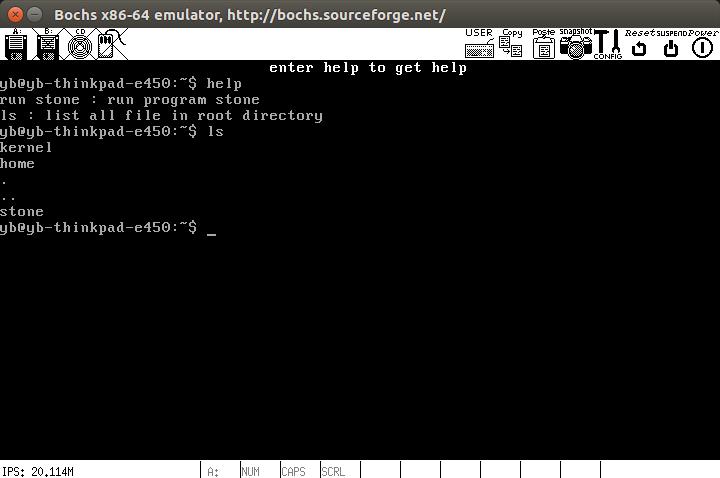
\includegraphics[scale=0.5]{asset/helpls.png}
        \caption{help和ls命令的截图\label{fig:helpls}} 
        \end{center} 
    \end{figure} 

    
    
    \begin{figure}[!htb]
        \begin{center}
        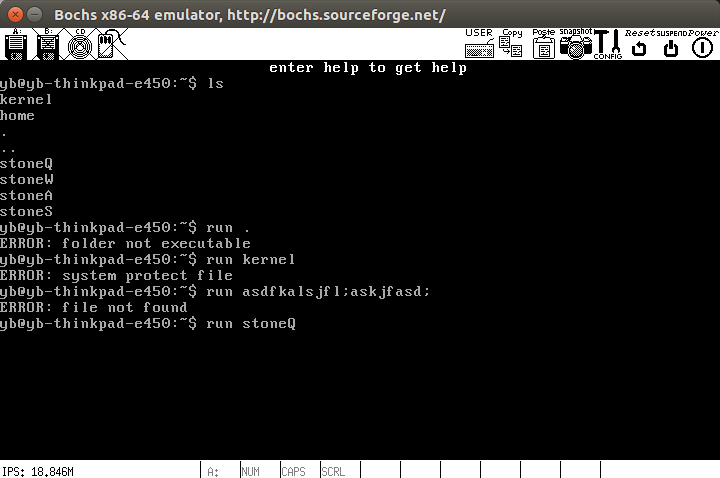
\includegraphics[scale=0.5]{asset/runfiles.png}
        \caption{run命令的截图\label{fig:runfiles}} 
        \end{center} 
    \end{figure} 
    
    
\section{实验总结}
    \subsection{亮点介绍}
    \subsubsection{makefile}
    项目按照更合理的方式分为各文件夹,并改用makefile的方式构建项目。为makefile提供了rebuild, clean, auto等指令,
    分别用于重新构筑项目,清空临时文件和自动构建并运行等操作。
    \subsubsection{GCC+NASM混合编程}
    成功地研究出了在Linux下使用GCC和NASM混编的方法。探索了C和汇编相互调用的各种困难,
    找到了他们的解决办法。\\

    我将混编的方法简单地总结成了一个模板,
    \\ 在网页 \url{https://github.com/YanB25/c-x86-hybrid-programming}
     上,可直接访问下载。该模板在Linux下可直接正确运行。其中王永锋同学还为该模板提供了Windows的环境。至此,该模板
     在支持全平台的开发。 \\

    \ref{subsec:GccNasmHybrid}节介绍了GCC和NASM混编成功的原理和本质原因。    \\
    \ref{subsec:gccnamspitfall} 节介绍了GCC和NASM混编时容易忽视的坑点难点,以及解决它们的办法。\\
    \ref{subsec:gccCompileIns}节详细地介绍了编译本个项目的所有编译选项,以及它们各自的作用。\\

    \subsubsection{文件系统}
    本项目超前地实现了FAT16文件系统。完成了基本的内核加载、文件读取、文件搜索、目录跳转等功能。
    \ref{sec:fsapi}节详细地介绍了文件系统的实现。
    \subsubsection{终端的实现}
    本项目实现了一个简单的终端,它支持输入help, ls, run等简单命令。它会对无法识别的命令报错。
    也会对无法运行的文件报错。终端支持退格键修改和删除命令。
    \subsubsection{简单printf实现}
    \ref{sec:library}节介绍了printf的实现。

    \subsection{心得体会}
    得益于实验延后了一周,我得以用这周的空档把文件系统的基础功能实现完。如果没有这一周的时间,我可能会选择
    不那么繁琐的A线路,先把中断给实现了。 \\
    
    这个实验最大的困难还是在第三周的混合编程上。Linux下的困难远比想象中的要大得多。实验三刚布置下来的几天里,
    我花了大量的时间研究编译指令及混编方法。熬了几次夜,但进展并不很顺利。我跟GCC+NASM讨论小组的
    同学都挺熟,那几天里我们做了很多很多的讨论。每个人都做过不同的尝试(当然也遇到了不同的失败)。
    当时我做的最坏打算是,这条路走不通,我就把所有的代码重构一遍,换windows下实验。所幸最后还是让
    我们找到了混编的方法,弄懂了失败的原因以及成功的原理。\\ 

    混编成功后,从``混编''到``完成IO函数库''间还有一小段空窗期。说空窗是因为,混编后,C语言生成的汇编代码的
    可读性并不太好,而此时IO函数又没有实现完,debug的手段比较有限。想用bochs调试C生成的汇编,需要有一定的耐心。
    所幸我在这一步中没有遇到很大的困难。随后的编程就很顺利了。有了C程序,还能利用IO将变量的值打印到屏幕上,调试
    变得简单了很多。\\
    
    在实现文件系统时也遇到了一些挫折。我最大的感想是,代码的编写,90\%以上是思考,10\%以下才是真正的代码编写。只有
    思考和学习后写出来的代码,才是更可靠的。
    \subsection{BUG总结} \label{sec:bug}
    写文件系统的FAT表时,struct元素初始化时漏写了一个元素,导致struct的元素``错位''了。由于没有指示GCC采用更
    严格的警告,GCC没有报出任何信息。FAT表的错误导致了操作系统的内核一直无法加载进内存。\\
    
    当时我困扰了比较久,因为扇区加载失败牵扯到的原因太多了。中断错误、寄存器的值错误、磁道数算错、内核没有写进虚拟镜像中……
    各种各样的原因我都排查后,我尝试把中间的各种变量都输出来,最后才找到了原因。 
\begin{appendices}
\section{参考文献} \label{sec:reference}
\begin{enumerate}
    \item https://blog.csdn.net/longintchar/article/details/50602851 \\
    16位和32位汇编指令的不同(尤其是push指令)
    \item https://www.ibiblio.org/gferg/ldp/GCC-Inline-Assembly-HOWTO.html\#s1 \\
    GCC 内嵌汇编的书写。
    \item http://blog.51cto.com/dengqi/1349327
    FAT32文件系统讲解
    \item https://blog.csdn.net/yeruby/article/details/41978199
    FAT16文件系统讲解
  \end{enumerate}
\section{其他代码} \label{sec:otherCode}
\begin{figure}
\begin{itemize}
\item[] \begin{lstlisting}[label=lst:wholepjtree, caption=项目总目录树]
.
├── bochsout.log
├── filesystem/
│   ├── API/
│   │   ├── fsapi.h
│   │   └── fsErrorCode.h
│   ├── datablock.c
│   ├── DBR.asm
│   ├── DBR.c
│   ├── FAT.c
│   ├── FATMacro.h
│   ├── filesystem.h
│   ├── fsutilities.asm
│   ├── fsutilities.h
│   ├── Makefile
│   └── README.md
├── include/
│   ├── bridge.inc
│   ├── graphic.h
│   ├── Makefile
│   ├── mystring.c
│   ├── mystring.h
│   ├── utilities.asm
│   └── utilities.h
├── kernel/
│   ├── kernel.c
│   ├── kernel.h
│   └── Makefile
├── loader/
│   ├── loader.asm
│   └── Makefile
├── Makefile
├── OS.img
└── user/
    ├── Makefile
    ├── stone
    ├── stone.c
    ├── stone.h
    ├── terminal.c
    ├── terminal.h
    ├── user.c
    └── user.h

7 directories, 34 files
\end{lstlisting}
\end{itemize}
\end{figure}
\end{appendices}
\end{document}